\documentclass{beamer}

\usepackage{beamerthemesplit}

\setbeamertemplate{footline}[page number]{}

\setbeamertemplate{navigation symbols}{}

\title{Getting Julia Ready for Statistical Computing}
\author{John Myles White}
\date{\today}

\begin{document}

\frame{\titlepage}

\frame
{
	\begin{center}
		Julia is a promising new language
	\end{center}
}

\frame
{
	\begin{center}
		At present, its strength is linear algebra, not data analysis
	\end{center}
}

\frame
{
	\begin{center}
		What do we need to start doing statistical computing in Julia?
	\end{center}
}

\frame
{
	Some examples:
	\begin{itemize}
		\item<1->{NA type (Harlan Harris)}
		\item<2->{DataFrame's (Harlan Harris)}
		\item<3->{Statistical distribution functions (Doug Bates)}
		\item<4->{GLM's (Doug Bates)}
		\item<5->{Hypothesis testing (JMW)}
		\item<6->{Optimization (JMW)}
	\end{itemize}
}

\frame
{
	\begin{center}
		 Let's talk about implementing optimization algorithms in Julia
	\end{center}
}

\frame
{
	\begin{center}
		Simulated Annealing is a randomized search method
	\end{center}
}

\frame
{
	\begin{center}
		SA is computationally intensive and a perfect candidate for Julia
	\end{center}
}

\begin{frame}[fragile]
	\begin{verbatim}
function simulated_annealing(cost::Function,
                             s0::Any,
                             neighbor::Function,
                             temperature::Function,
                             iterations::Int64,
                             keep_best::Bool
                             
  # Set our current state to the specified intial state.
  s = s0

  # Set the best state we've seen to the intial state.
  best_s = s0
	\end{verbatim}
\end{frame}

\begin{frame}[fragile]
	\begin{verbatim}
  # We always perform a fixed number of iterations.
  for i = 1:iterations
  
    # Find the proper temperature at time i.
    t = temperature(i)
    
    # Randomly generate a neighbor of our current state.
    s_n = neighbor(s)
    
    # Evaluate the cost function.
    y = cost(s)
    y_n = cost(s_n)
    	\end{verbatim}
\end{frame}

\begin{frame}[fragile]
	\begin{verbatim}    
    if y_n <= y
      # We always move to superior states.
      s = s_n
    else
      # We probabilistically move to inferior states.
      p = exp(- ((y_n - y) / t))
            
      if rand() <= p
        s = s_n
      else
        s = s
      end
    end
    	\end{verbatim}
\end{frame}

\begin{frame}[fragile]
	\begin{verbatim}    
    # Keep a record of the best state we've seen.
    if cost(s) < cost(best_s)
      best_s = s
    end
  end
  
  # Return the best state or the last state we've seen.
  if keep_best
    best_s
  else
    s
  end
end
	\end{verbatim}
\end{frame}

\frame
{
	\begin{center}
		That very generic code runs quite fast in Julia
	\end{center}
}

\begin{frame}[fragile]
	\begin{verbatim}
function rosenbrock(x, y)
  (1 - x)^2 + 100(y - x^2)^2
end
 
function neighbors(z)
  [rand_uniform(z[1] - 1, z[1] + 1),
   rand_uniform(z[2] - 1, z[2] + 1)]
end
 
simulated_annealing(z -> rosenbrock(z[1], z[2]),
                    [0, 0],
                    neighbors,
                    i -> 1 / log(i),
                    10000,
                    true)
	\end{verbatim}
\end{frame}

\frame
{
	\begin{center}
		We can run this thousands of times to see how well it performs
	\end{center}
}

\frame
{
	\begin{center}
		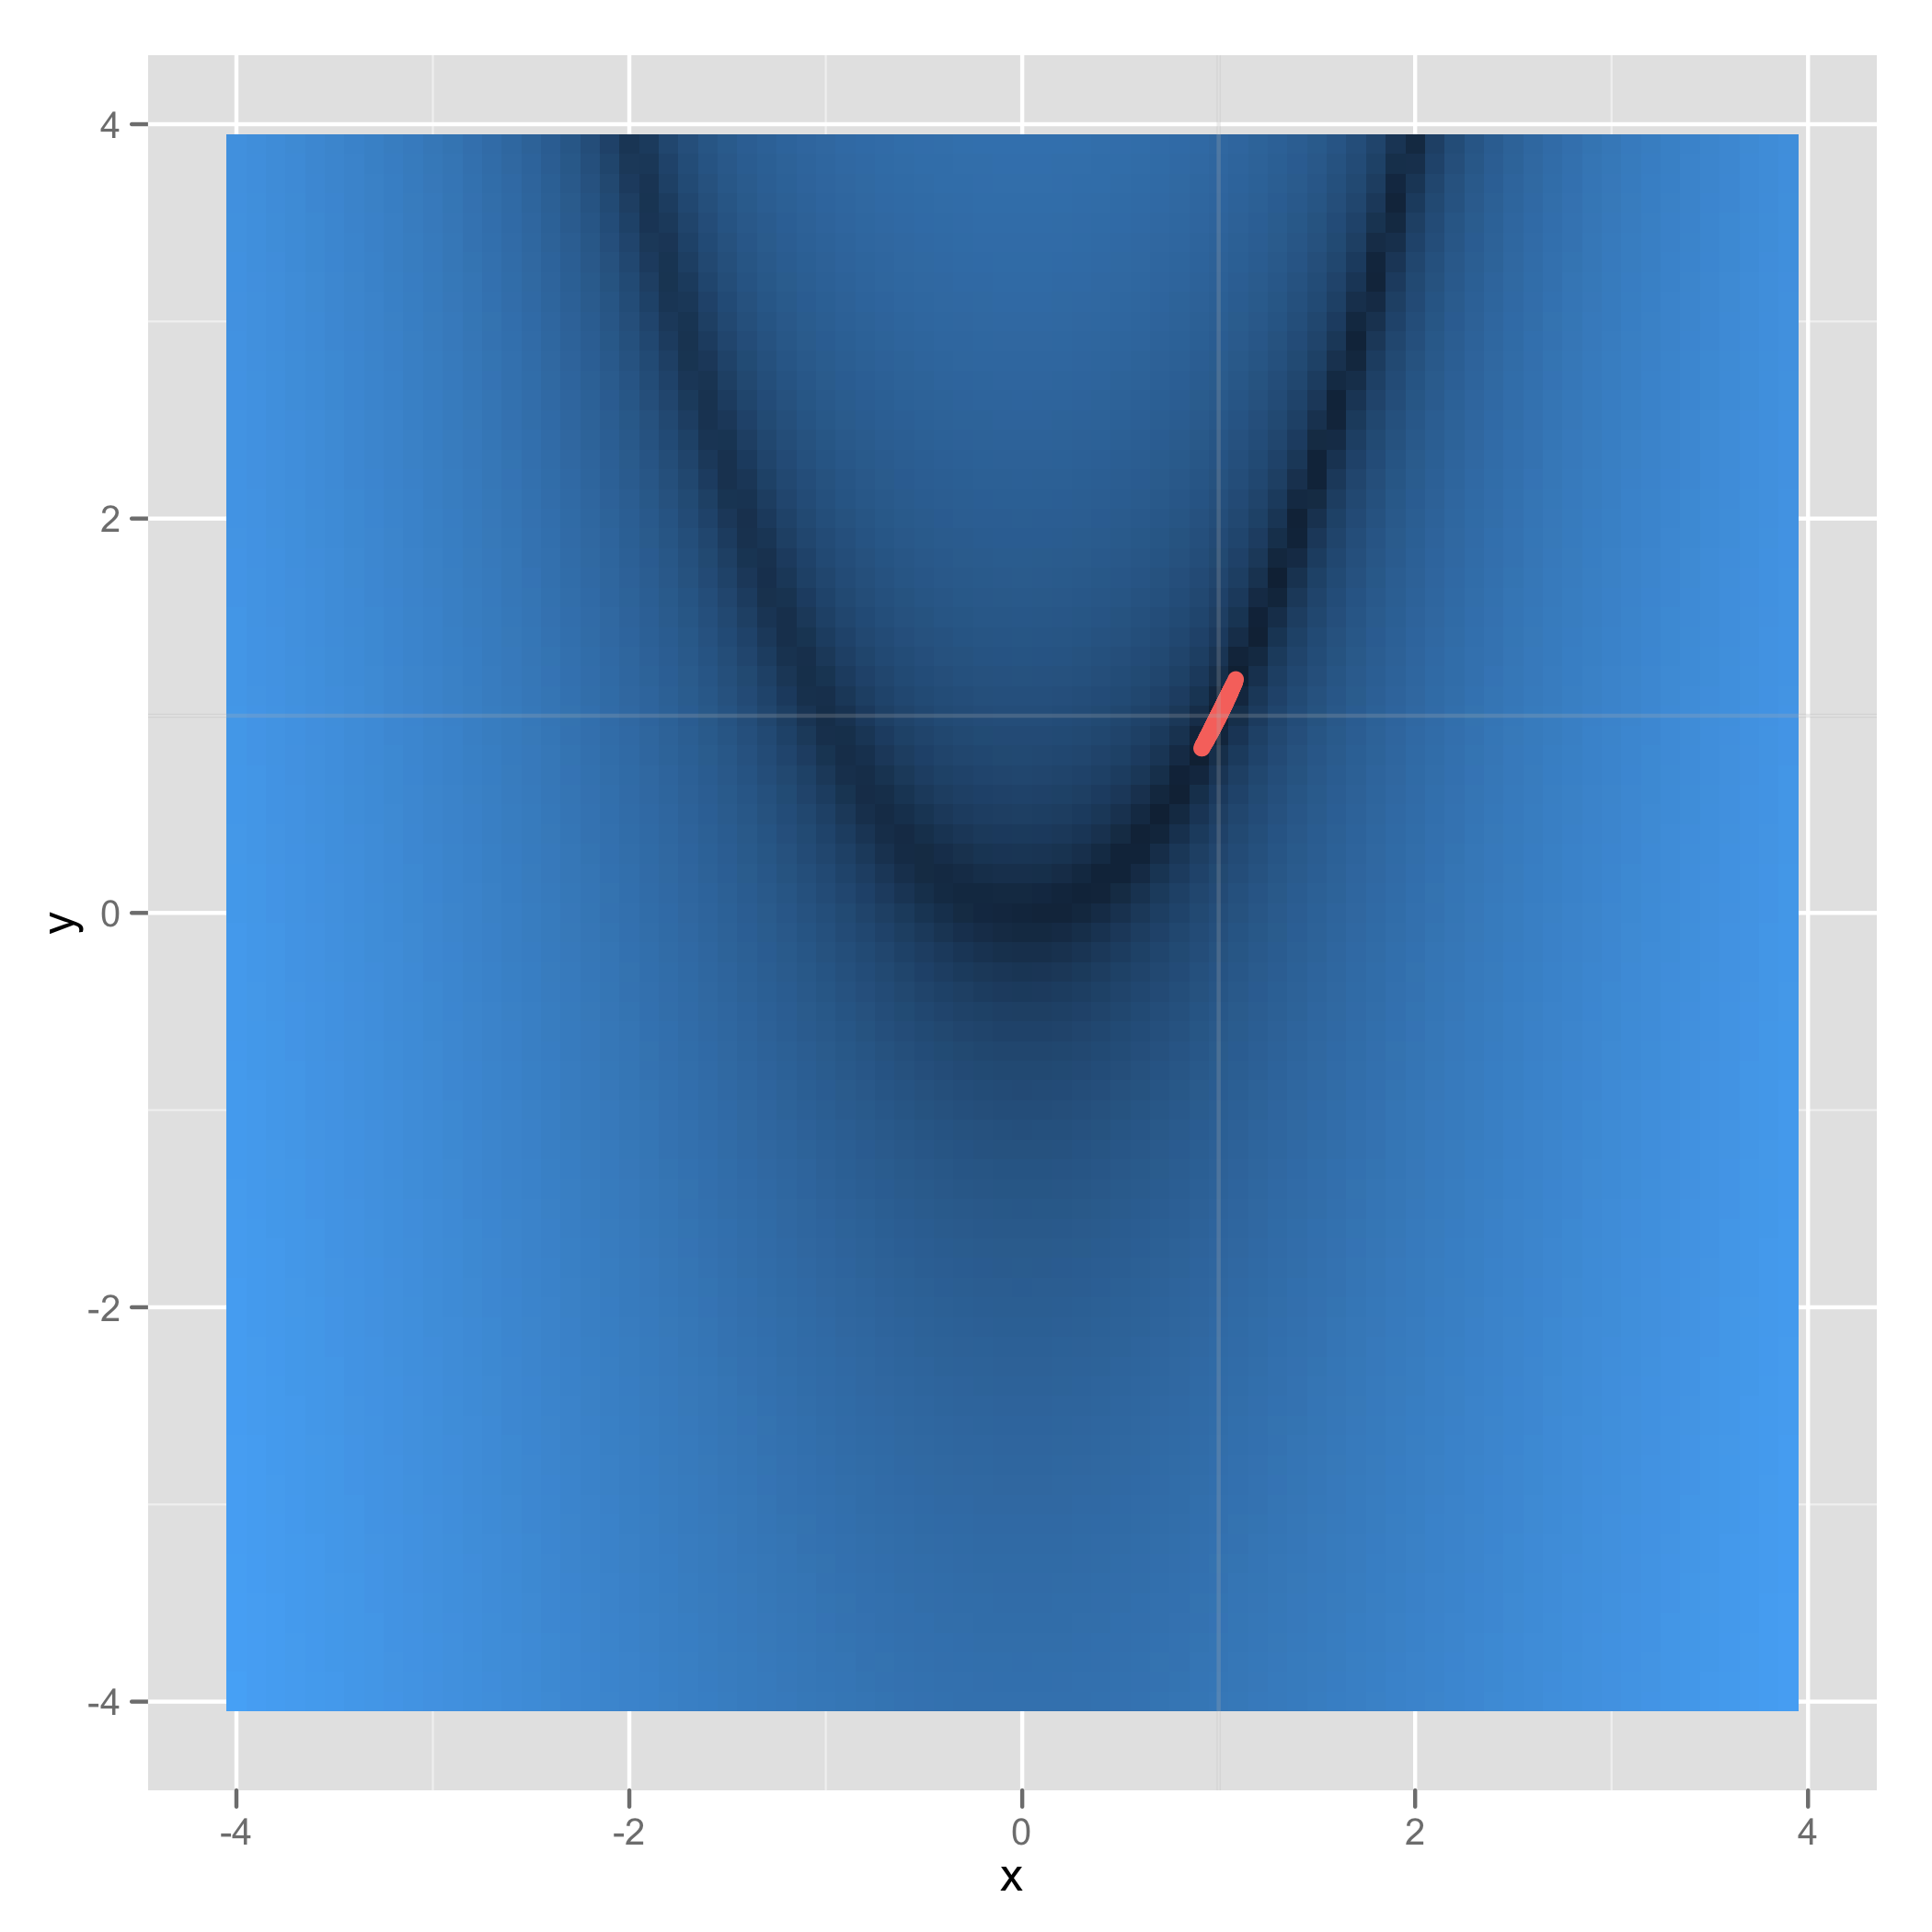
\includegraphics[scale = 0.1]{rosenbrock.png}
	\end{center}
}

\frame
{
	\begin{center}
		We can also estimate average run-time of 10,000 iterations
	\end{center}
}

\begin{frame}[fragile]
	\begin{verbatim}
@elapsed for i = 1:5000
  simulated_annealing(z -> rosenbrock(z[1], z[2]),
                      [0, 0],
                      neighbors,
                      i -> 1 / log(i),
                      10000,
                      true)
end
	\end{verbatim}
\end{frame}

\frame
{
	\begin{center}
		Each run of 10,000 iterations takes about 25 milliseconds
	\end{center}
}

\frame
{
	\begin{center}
		Julia has a lot of promise, but it needs you
	\end{center}
}

\frame
{
	\begin{center}
		Julia needs people to implement algorithms
	\end{center}
}

\frame
{
	\begin{center}
		Julia needs feedback on language design
	\end{center}
}

\end{document}
